\documentclass{article}
\usepackage[english]{babel}
\usepackage{amssymb,graphicx,hyperref,alltt}

%%%%%%%%%% Start TeXmacs macros
\newcommand{\tmaffiliation}[1]{\\ #1}
\newcommand{\tmtextit}[1]{{\itshape{#1}}}
\newcommand{\tmtexttt}[1]{{\ttfamily{#1}}}
\newenvironment{tmcode}[1][]{\begin{alltt} }{\end{alltt}}
%%%%%%%%%% End TeXmacs macros

\begin{document}

\title{Computational physics}

\author{
  Youjun Hu
  \tmaffiliation{Institute of Plasma Physics, Chinese Academy of Sciences}
  \tmaffiliation{Email: yjhu@ipp.cas.cn}
}

\maketitle

\section{Introduction}

Physics becomes concrete, impressive, and fun when we compute it numerically
and visualize the process by graphics. Computational physics are primarily
about numerically solving three types of partial differential equations
(PDEs), namely hyperbolic, parabolic, and elliptic PDEs, which respectively
correspond to advection (wave) equations, diffusion equations, and Poisson's
equations.

\section{Advection equation}

In one-dimensional case, an advection equation takes the following form:
\begin{equation}
  \frac{\partial y}{\partial t} = - c \frac{\partial y}{\partial x},
\end{equation}
where $c$ is a constant. A natural choice of differencing scheme for the above
equation is
\begin{equation}
  \frac{y_i^{(n + 1)} - y_i^{(n)}}{\Delta t} = \frac{y_{(i + 1)}^{(n)} - y_{(i
  - 1)}^{(n)}}{2 \Delta x},
\end{equation}
which however is unconditionally unstable (tested by me numerically. the
stability analysis can prove that the above scheme is unconditional
unstable{\cite{Fitzpatrickcp}}). The Lax-Friedrichs scheme modifies the above
scheme to the following form:
\begin{equation}
  \frac{y_i^{(n + 1)} - \frac{y_{ (i - 1)}^{(n)} + y_{(i +
  1)}^{(n)}}{2}}{\Delta t} = - c \frac{y_{(i + 1)}^{(n)} - y_{(i -
  1)}^{(n)}}{2 \Delta x},
\end{equation}
which is stable if the CFL condition is satisfied. However this scheme
introduces heavy damping in the solution, as is shown in Fig \ref{18-4-9-2}.
The Lax-Friedrichs scheme is an explicit scheme. Let us try implicit schemes.
One natural choice of implicit scheme is of the following form:
\begin{equation}
  \label{18-4-8-1} \frac{y_i^{(n + 1)} - y_i^{(n)}}{\Delta t} = - \frac{1}{2}
  c \left[ \frac{y_{(i + 1)}^{(n + 1)} - y_{(i - 1)}^{(n + 1)}}{2 \Delta x} +
  \frac{y_{(i + 1)}^{(n)} - y_{(i - 1)}^{(n)}}{2 \Delta x} \right],
\end{equation}
which is called the Crank--Nicolson implicit scheme. An implicit scheme
usually requires that an linear equations system be solved because the unknown
future values are usually coupled together. The scheme (\ref{18-4-8-1}) can be
organized in the following form
\begin{equation}
  y_i^{(n + 1)} + \frac{\Delta t}{2} c \left[ \frac{y_{(i + 1)}^{(n + 1)} -
  y_{(i - 1)}^{(n + 1)}}{2 \Delta x} \right] = y_i^{(n)} - \frac{\Delta t}{2}
  c \left[ \frac{y_{(i + 1)}^{(n)} - y_{(i - 1)}^{(n)}}{2 \Delta x} \right],
\end{equation}
which is a traditional equation system. Figure \ref{18-4-9-2} compares the
results calculated by the Lax-Friedrichs scheme and the Crank--Nicolson
scheme, which shows that no damping is introduced by the Crank-Nicolson
scheme.

\begin{figure}[h]
  \resizebox{8cm}{!}{\includegraphics{/home/yj/project_new/1d_advection/fig1/p.eps}}\resizebox{8cm}{!}{\includegraphics{/home/yj/project_new/1d_advection_crank_nicholson/fig1/p.eps}}
  \caption{\label{18-4-9-2}Evolution of the waveform computed by the
  Lax-Friedrichs scheme (left) and the Crank--Nicolson implicit scheme
  (right). Simulations are performed with the Initial condition given by $y
  (x, t = 0) = \exp (- 100 (x - 0.5)^2)$, time-step size $d t = 0.05 d x / c$,
  grid spacing $d x = 1 / (N_x - 1)$, $N_x = 200$. Both schemes give correct
  the propagation speed, but the Lax-Friedrichs scheme introduces heavy
  damping in the solution.}
\end{figure}

\

\

\section{Wave equation}

A wave equation in one-dimension takes the following form:
\begin{equation}
  \label{18-4-15-1} \frac{\partial^2 y}{\partial t^2} = c \frac{\partial^2
  y}{\partial x^2},
\end{equation}
which is a second order differential equation and can be written as two
coupled advection equations. Define a new function $\xi$ by
\begin{equation}
  \label{18-4-15-2} \frac{\partial \xi}{\partial t} = \frac{\partial
  y}{\partial x}
\end{equation}
Then Eq. (\ref{18-4-15-1}) can be written as
\begin{equation}
  \frac{\partial^2 y}{\partial t^2} = c \frac{\partial \xi}{\partial t
  \partial x},
\end{equation}
which can be simplified as
\begin{equation}
  \label{18-4-15-3}  \frac{\partial y}{\partial t} = c \frac{\partial
  \xi}{\partial x} .
\end{equation}
Equation (\ref{18-4-15-2}) and (\ref{18-4-15-3}) are two couple advection
equations.

\subsection{Maxwell's equation in 1D case}

For Maxwell's equation in one-dimension case, there are two independent TEM
modes, one of which is described by
\begin{equation}
  \frac{\partial B_y}{\partial t} = \frac{\partial E_z}{\partial x},
\end{equation}
\begin{equation}
  \frac{\partial E_z}{\partial t} = c^2 \frac{\partial B_y}{\partial x},
\end{equation}
where $c = 1 / \sqrt{\mu_0 \varepsilon_0}$ is the speed of light in vacuum. In
an electromagnetic wave, $E_z$ is $c$ times of $B_z$ in SI units. To make the
two variables in the above equation takes similar magnitude, define
$\overline{E}_z = E_z / c$. Then using $(\overline{E}_z, B_y)$ as variables,
the above equations are written
\begin{equation}
  \label{18-4-15-4} \frac{\partial B_y}{\partial t} = c \frac{\partial
  \overline{E}_z}{\partial x},
\end{equation}
\begin{equation}
  \label{18-4-15-5} \frac{\partial \overline{E}_z}{\partial t} = c
  \frac{\partial B_y}{\partial x},
\end{equation}

\subsection{The Lax scheme}

Similar to the case of advection equation, the following simple differencing
scheme for the vacuum TEM equations (\ref{18-4-15-4}) and (\ref{18-4-15-5}):
\begin{equation}
  \frac{B_{y i}^{(n + 1)} - B_{y i}^{(n)}}{\Delta t} = c \frac{\overline{E}_{z
  (i + 1)}^{(n)} - \overline{E}_{z (i - 1)}^{(n)}}{2 \Delta x} .
\end{equation}

\begin{equation}
  \frac{\overline{E}_{z i}^{(n + 1)} - \overline{E}_{z i}^{(n)}}{\Delta t} = c
  \frac{B_{y (i + 1)}^{(n)} - B_{y (i - 1)}^{(n)}}{2 \Delta x} .
\end{equation}
is unstable (tested numerically by me). The Lax scheme modifies the above
scheme to the following form:


\begin{equation}
  \frac{B_{y i}^{(n + 1)} - \frac{B_{y (i - 1)}^{(n)} + B_{y (i +
  1)}^{(n)}}{2}}{\Delta t} = c \frac{\overline{E}_{z (i + 1)}^{(n)} -
  \overline{E}_{z (i - 1)}^{(n)}}{2 \Delta x} .
\end{equation}

\begin{equation}
  \frac{\overline{E}_{z i}^{(n + 1)} - \frac{\overline{E}_{z (i - 1)}^{(n)} +
  \overline{E}_{z (i + 1)}^{(n)}}{2}}{\Delta t} = c \frac{B_{y (i + 1)}^{(n)}
  - B_{y (i - 1)}^{(n)}}{2 \Delta x} .
\end{equation}
I tested this and found it induces heavy damping as it does in the case of
advection equation.

\subsection{The Crank--Nicolson scheme}

Let us try the Crank-Nicolson implicit scheme:


\begin{equation}
  \frac{B_{y (i)}^{(n + 1)} - B_{y (i)}^{(n)}}{\Delta t} = \frac{1}{2} c
  \left( \frac{\overline{E}_{z (i + 1)}^{(n + 1)} - \overline{E}_{z (i -
  1)}^{(n + 1)}}{2 \Delta x} + \frac{\overline{E}_{z (i + 1)}^{(n)} -
  \overline{E}_{z (i - 1)}^{(n)}}{2 \Delta x} \right),
\end{equation}
\begin{equation}
  \frac{\overline{E}_{z (i)}^{(n + 1)} - \overline{E}_{z (i)}^{(n)}}{\Delta t}
  = \frac{1}{2} c \left( \frac{B_{y (i + 1)}^{(n + 1)} - B_{y (i - 1)}^{(n +
  1)}}{2 \Delta x} + \frac{B_{y (i + 1)}^{(n)} - B_{y (i - 1)}^{(n)}}{2 \Delta
  x} \right) .
\end{equation}
The above differencing scheme can be organized in the following form:


\begin{equation}
  B_{y (i)}^{(n + 1)} - \frac{\Delta t}{2} c \left( \frac{\overline{E}_{z (i +
  1)}^{(n + 1)} - \overline{E}_{z (i - 1)}^{(n + 1)}}{2 \Delta x} \right) =
  \frac{\Delta t}{2} c \left( \frac{\overline{E}_{z (i + 1)}^{(n)} -
  \overline{E}_{z (i - 1)}^{(n)}}{2 \Delta x} \right) + B_{y (i)}^{(n)},
\end{equation}
\begin{equation}
  \overline{E}_{z (i)}^{(n + 1)} - \frac{\Delta t}{2} c \left( \frac{B_{y (i +
  1)}^{(n + 1)} - B_{y (i - 1)}^{(n + 1)}}{2 \Delta x} \right) = \frac{\Delta
  t}{2} c \left( \frac{B_{y (i + 1)}^{(n)} - B_{y (i - 1)}^{(n)}}{2 \Delta x}
  \right) + \overline{E}_{z (i)}^{(n)} .
\end{equation}
which is a linear equation system for $(B_{y i}^{(n + 1)}, \overline{E}_{z
i}^{(n + 1)})$ with $i = 1, 2, \ldots N_x$, where $N_x$ is the number of grids
in the $x$ direction. This linear system is solved by using LU decomposition
of the coefficient matrix (the LU decomposition can be viewed as the matrix
form of Gaussian elimination.). The evolution of the wave form calculated by
this scheme is plotted in Fig. \ref{18-4-9-1}.

\begin{figure}[h]
  \resizebox{8cm}{!}{\includegraphics{/home/yj/project_new/1d_TEM_wave/fig1/p.eps}}\resizebox{8cm}{!}{\includegraphics{/home/yj/project_new/1d_TEM_wave/fig2/p.eps}}
  \caption{\label{18-4-9-1}Evolution of the TEM waveform $(B_y, E_z)$ computed
  by the Crank--Nicolson implicit scheme. Simulations are performed with the
  initial condition $E_z (x, t = 0) = 0$, $B_y (x, t = 0) = \exp (- (x -
  x_0)^2 / (0.1 L)^2)$, $x_0 = 0.5 m$, $L = 1 m$, time-step size $d t = 0.01 d
  x / c$, grid spacing $d x = 1 / (N_x - 1)$, $N_x = 100$. Fixed zero boundary
  condition is used: $E_z (x = 0) = E_z (x = L) = 0$, $B_y (x = 0) = B_y (x =
  L) = 0$. Since the waveform has not reach the boundary, the boundary has no
  effect on the evolution. The results show that two traveling waves emerge
  from the Gaussian waveform of $B_y$, propagating in the opposite directions.
  The propagation speed is correct.}
\end{figure}

\

\section{Diffusion equation}

The stencil used in the explicit, implicit, and Crank--Nicolson implicit
method is given in Figure (\ref{18-4-15-8}).

\

\begin{figure}[h]
  \resizebox{5cm}{!}{\includegraphics{/home/yj/theory/figures/implicit_scheme/explicit-1.eps}}\resizebox{5cm}{!}{\includegraphics{/home/yj/theory/figures/implicit_scheme/explicit-2.eps}}\resizebox{5cm}{!}{\includegraphics{/home/yj/theory/figures/implicit_scheme/explicit-3.eps}}
  \caption{\label{18-4-15-8}Stencil of an explicit scheme (left) implicit
  scheme (middle) and the Crank-Nicolson implicit scheme (right) for the
  diffusion equation $u_t = u_{x x}$.}
\end{figure}

This part is to be continued.

\

\section{Poisson's equation}

Poisson's equation is written
\begin{equation}
  \nabla^2 \varphi = S,
\end{equation}
where $S$ is a known source term. In Cartesian coordinates and in the 2D case,
the above equation is written
\begin{equation}
  \frac{\partial^2 \varphi}{\partial x^2} + \frac{\partial^2 \varphi}{\partial
  x^2} = S (x, y) .
\end{equation}
Consider solving the above equation in a rectangular domain with $x_a
\leqslant x \leqslant x_b$ and $y_a \leqslant y \leqslant y_b$ and with
$\varphi = 0$ on the boundary.

\subsection{Discretized form using finite differencing}

Discretize $x$ as $x_i = x_a + (i + 1) \Delta_x$, where $\Delta_x = (x_b -
x_a) / (M + 1)$ and $i = 0, 1, 2, \ldots, M - 1$. Similarly, discretize $y$ as
$y_j = y_a + (j + 1) \Delta_y$, where $\Delta_y = (y_b - y_a) / (N + 1)$ and
$j = 0, 1, 2, \ldots, N - 1$. Then the above equation can be discretized by
using the following finite difference:
\begin{equation}
  \label{18-7-21-p1} \frac{\varphi_{i + 1, j} - 2 \varphi_{i, j} + \varphi_{i
  - 1, j}}{\Delta^2_x} + \frac{\varphi_{i, j + 1} - 2 \varphi_{i, j} +
  \varphi_{i, j - 1}}{\Delta^2_y} = S_{i, j},
\end{equation}
where $\varphi_{i, j} = \varphi (x_i, y_j)$ and $S_{i, j} = S (x_i, y_j)$.
Equation (\ref{18-7-21-p1}) can be arranged as
\begin{equation}
  \label{18-7-21-p2} a \varphi_{i + 1, j} + a \varphi_{i - 1, j} + c
  \varphi_{i, j} + b \varphi_{i, j + 1} + b \varphi_{i, j - 1} = S_{i, j},
\end{equation}
where $a = 1 / \Delta_x^2$, $b = 1 / \Delta_y^2$, and $c = - \left(
\frac{2}{\Delta_x^2} + \frac{2}{\Delta_y^2} \right)$. This is a 5-points
stencil, as is illustrated in Fig. \ref{18-7-21-p4}.

\begin{figure}[h]
  \resizebox{5cm}{!}{\includegraphics{/home/yj/theory/figures/ordering/5point-1.eps}}
  \caption{\label{18-7-21-p4}Five-points stencil of the finite differencing
  scheme in Eq. (\ref{18-7-21-p2}).}
\end{figure}

\

In this discritization, the boundary conditions are written as $\varphi_{- 1,
j} = \varphi_{M, j} = 0$ and $\varphi_{i, - 1} = \varphi_{i, N} = 0$.

\subsection{Matrix form of the difference scheme}

In order to solve the linear equation system (\ref{18-7-21-p2}), we prefer to
formulate it in a matrix form. In order to do this, we need to order the 2D
discrete unknowns $\varphi_{i, j}$ in a 1D sequence. Two natural ordering
schemes are the row-ordering and the column ordering. I choose the row
ordering, as is illustrated in Fig. \ref{18-7-21-1}.

\begin{figure}[h]
  \resizebox{10cm}{!}{\includegraphics{/home/yj/theory/figures/ordering/ordering-1.eps}}
  \caption{\label{18-7-21-1}Row-ordering of the 2D discrete unknowns
  $\varphi_{i, j}$ on a $3 \times 3$ mesh.}
\end{figure}

Using the above ordering, the linear equation system (\ref{18-7-21-p2}) for
the special case of a $3 \times 3$ mesh is written as the following matrix
form:
\begin{equation}
  \left(\begin{array}{ccccccccc}
    c & a &  & b &  &  &  &  & \\
    a & c & a &  & b &  &  &  & \\
    & a & c &  &  & b &  &  & \\
    b &  &  & c & a &  & b &  & \\
    & b &  & a & c & a &  & b & \\
    &  & b &  & a & c &  &  & b\\
    &  &  & b &  &  & c & a & \\
    &  &  &  & b &  & a & c & a\\
    &  &  &  &  & b &  & a & c
  \end{array}\right) \left(\begin{array}{c}
    \varphi_0\\
    \varphi_1\\
    \varphi_2\\
    \varphi_3\\
    \varphi_4\\
    \varphi_5\\
    \varphi_6\\
    \varphi_7\\
    \varphi_8
  \end{array}\right) = \left(\begin{array}{c}
    S_0\\
    S_1\\
    S_2\\
    S_3\\
    S_4\\
    S_5\\
    S_6\\
    S_7\\
    S_8
  \end{array}\right),
\end{equation}
where all the blank elements are zeros. This $9 \times 9$ matrix is sparse but
is not triangular. Each row of the matrix corresponds to one difference
equation at a grid point. It is not difficult to generalize the above $9
\times 9$ matrix to a general $M N \times M N$ matrix. The general pattern is
that those rows that corresponds to inner grid points have the following
pattern $(\ldots, b, \ldots, a, c, a, \ldots, b, \ldots)$, where $c$ is on the
diagonal location and the distance between $b$ and $c$ is $M$. For those rows
that correspond to boundary grid points, some $b$ and/or $a$ can be absent.
Specifically, (1) the left $a$ is absent for all the rows corresponding to the
left boundary grids; (2) the right $a$ is absent for all the rows
corresponding to the right boundary grids; (3) the left $b$ is absent for all
the rows corresponding to bottom boundary grids; (4) the right $b$ is absent
for all the rows corresponding to the top boundary grids. The following Fotran
code illustrates how to set up the matrix elements for this kind of sparse
matrix:
\begin{tmcode}
dx=1.0/(m+1)
dy=1.0/(n+1)
a_coef= 1./dx**2
b_coef=1./dy**2
c_coef = -2*(a_coef+b_coef)
A=0 !initialize coefficent matrix
do  II=0,m*n-1
     A(II,II)=c_coeff !diagonal elements
     j = II/m !recover the original index in the y direction of the 2D mesh
     if (j.gt.0) A(II,II-m)=b_coef
     if (j.lt.n-1) A(II,II+m)=b_coeff
     i = II - j*m !recover the original index in the x direction of the 2D mesh
     if (i.gt.0) A(II,II-1)=a_coeff
     if (i.lt.m-1) A(II,II+1)=a_coeff
enddo
\end{tmcode}
I use PETSc parallel library{\cite{petsc-web-page}} to solve the above linear
system. In this case, the corresponding code for setting up the matrix in
parallel is as follows:
\begin{tmcode}
dx=1.0/(m+1)
dy=1.0/(n+1)
a_coef= 1./dx**2
b_coef=1./dy**2
c_coef = -2*(a_coef+b_coef)
call MatGetOwnershipRange(A,Istart,Iend,ierr) 
do  II=Istart,Iend-1
     call  MatSetValues(A,ione,II,ione,II,c_coef,INSERT_VALUES,ierr) !diagonal elements

     j = II/m !recover the original index in the y direction of the 2D mesh
     if (j.gt.0) then
        JJ = II - m
        call MatSetValues(A,ione,II,ione,JJ,b_coef,INSERT_VALUES,ierr)
     endif
     if (j.lt.n-1) then
        JJ = II + m
        call MatSetValues(A,ione,II,ione,JJ,b_coef,INSERT_VALUES,ierr)
     endif
  
    i = II - j*m !recover the original index in the x direction of the 2D mesh
     if (i.gt.0) then
        JJ = II - 1
        call MatSetValues(A,ione,II,ione,JJ,a_coef,INSERT_VALUES,ierr)
     endif
     if (i.lt.m-1) then
        JJ = II + 1
        call MatSetValues(A,ione,II,ione,JJ,a_coef,INSERT_VALUES,ierr)
     endif
enddo
call MatAssemblyBegin(A,MAT_FINAL_ASSEMBLY,ierr)
call MatAssemblyEnd  (A,MAT_FINAL_ASSEMBLY,ierr)
\end{tmcode}
All the elements that are not updated by \tmtexttt{MatSetValues} in the above
code are by default zero.

\subsection{Verification of the numerical solution}

For the particular source term given by
\begin{equation}
  S (x, y) = \sin (\pi x) \sin (\pi y),
\end{equation}
then
\begin{equation}
  \varphi (x, y) = - \frac{1}{2 \pi^2} \sin (\pi x) \sin (\pi y),
\end{equation}
satisfies the equation and the boundary condition $\psi = 0$ at $x_a = 0$,
$x_b = 1$, $y_a = 0$, and $y_b = 1$. Therefore the above expression is an
analytic solution to the problem. Figure \ref{2018-7-23-a1} compares the
numerical solution with the analytic one, which indicates the two results
agree with each other, and thus verifying the correctness of the numerical
solution.

\begin{figure}[h]
  \includegraphics{/home/yj/project_new/petsc_space/poisson/p.eps}
  \caption{\label{2018-7-23-a1}Comparison between the numerical solution and
  analytic solution of Poisson' equation. Numerical parameters: grid number $M
  = 50$, $N = 50$. The resulting linear system has $2500$ unknowns. PETSc
  provides a flexible way of choosing different algorithms for solving the
  linear system via command line options. The command line options used for
  this case is: \tmtexttt{mpiexec -n 3 ./poisson -pc\_type bjacobi
  -sub\_pc\_type ilu -ksp\_type bcgs -ksp\_monitor}, which chooses the
  preconditioner type and Krylov subspace method type. The KSP residual norm
  is $1.456 \times 10^{- 7}$ after 25 iterations.}
\end{figure}

\

\section{A simple example of numerical instability}

For the following ordinary differential equation:
\begin{equation}
  \frac{d y}{d t} = - a y,
\end{equation}
where $a$ is a positive constant, with the initial condition $y (0) = y_0$,
the analytic solution is given by
\begin{equation}
  \label{18-4-11-p3} y = y_0 \exp (- a t),
\end{equation}
which is a monotonically decreasing function of $t$. Let us try to solve this
initial value problem numerically. Discritizing time as \ $t_n = n \Delta t$
with $\Delta t > 0$, we use the following explicit differencing scheme:
\begin{equation}
  \frac{y^{(n + 1)} - y^{(n)}}{\Delta t} = - a y^{(n)},
\end{equation}
i.e.,
\begin{equation}
  \label{18-4-11-1} y^{(n + 1)} = (1 - \Delta t a) y^{(n)},
\end{equation}
where $y^{(n)} = y (t_n)$ and $y^{(n + 1)} = y (t_{n + 1})$. If we choose a
large time-step $\Delta t$ with $\Delta t > 2 / a$, then $| 1 - \Delta t a | >
1$ and the above scheme gives a numerical solution with amplitude increasing
with time, instead of decaying. This is totally different from the analytic
solution, which indicates the numerical solution is wrong in this case. This
kind of wrong numerical solution is called a numerical instability. An example
is shown in Fig. \ref{18-4-11-2}.

\begin{figure}[h]
  \resizebox{8cm}{!}{\includegraphics{/home/yj/project_new/numerical_instability/fig1/f.eps}}
  \caption{\label{18-4-11-2}Comparison between the analytic solution
  (\ref{18-4-11-p3}) (black) and the numerical solution (blue) calculated by
  the scheme (\ref{18-4-11-1}) with $\Delta t = 2.1$. Other parameters: $y_0 =
  1$, $a = 1$.}
\end{figure}

\

Let us consider the following implicit scheme
\begin{equation}
  \frac{y^{(n + 1)} - y^{(n)}}{\Delta t} = - a y^{(n + 1)},
\end{equation}
(where the right-hand side is evaluated at the future time time), i.e.,
\begin{equation}
  \label{18-4-11-p1} y^{(n + 1)} = \frac{y^{(n)}}{1 + a \Delta t} .
\end{equation}
Note that no matter how large the time step-length $\Delta t$ is, the above
scheme always give a solution which is decreasing with time, i.e., no
numerical instability appears. An example is shown in Fig. \ref{18-4-11-p2}.

\begin{figure}[h]
  \resizebox{8cm}{!}{\includegraphics{/home/yj/project_new/numerical_instability/fig2/f.eps}}
  \caption{\label{18-4-11-p2}Comparison between the analytic solution
  (\ref{18-4-11-p3}) (black) and the numerical solution (blue) calculated by
  the scheme (\ref{18-4-11-p1}) with $\Delta t = 2.1$. Other parameters: $y_0
  = 1$, $a = 1$.}
\end{figure}

If a one-step explicit scheme is unstable, then the corresponding implicit
scheme is stable. This is because that an implicit scheme corresponds to a
time-reversed version of the corresponding explicit scheme.

\

\section{Finite difference}

Taylor expansion of $f (x)$ at $x = x_i$ is written as
\begin{equation}
  f (x_i + h) = f (x_i) + h f^{(1)} (x_i) + \frac{h^2}{2} f^{(2)} (x_i) + O
  (h^3)
\end{equation}


\section{The predictor-corrector method}

This method is very similar to and often confused with the Runge-Kutta method.
Consider the following differential equation
\begin{equation}
  \frac{d y}{d t} = f (y)
\end{equation}
A natural discretized form that is time-centered would be
\begin{equation}
  y_{n + 1} = y_n + \frac{\Delta t}{2} [f (y_{n + 1}) + f (y_n)] .
\end{equation}
Unfortunately the presence of $y_{n + 1}$ on the right-hand side makes this
scheme implicit, and thus a direct solution is possible only for some special
cases (e.g. $f (y)$ is a linear function of $y$). Generally, we need to use
iterations to solve the above equation. A convenient initial guess is $y_{n +
1} \approx y_n$. If we iterate for only twice, i.e.,
\begin{equation}
  y_{n + 1}^{(1)} = y_n + \Delta t f (y_n)
\end{equation}
\begin{equation}
  y_{n + 1}^{(2)} = y_n + \frac{\Delta t}{2} [f (y_{n + 1}^{(1)}) + f (y_n)] .
\end{equation}
Then this is the predictor-corrector method (also called Heun's method). This
method consists of a guess for $y_{n + 1}$ based on the Euler method (the
Prediction) followed by a correction using trapezoidal rule.

If we iterate until convergence, then this is a general implicit scheme.

\

\

\section{Spectral method-----to be revised}

Spectral methods refers to methods of using linear combination of global basis
functions to approximate a unknown function. Here ``global'' means that the
basis functions extending over the whole spatial domain of interest, i.e., has
a support as large as the whole domain of interest (contrast to the finite
element method, which use local basis functions). Here we consider Fourier
spectral method, which uses trigonometric functions as basis functions.
Consider the following two-point boundary value problem:
\begin{equation}
  \label{18-1-24-p1} L \psi (x) \equiv \left[ - \frac{\partial^2}{\partial
  x^2} + V (x) \right] \psi (x) = S (x),
\end{equation}
with the boundary condition $\psi (x = L) = \psi (x = 0)$, where $V (x)$ and
$S (x)$ are known functions. Expand $\psi (x)$ in terms of the Fourier basis
functions:
\begin{equation}
  \psi (x) \approx \sum_{n = 0}^{N - 1} \hat{\psi}_n \exp \left( n \frac{2 \pi
  i x}{L} \right),
\end{equation}
where $\hat{\psi}_n$ are unknown coefficients. Substitute this expression into
the left-hand side of Eq. (\ref{18-1-24-p1}), we obtain
\begin{eqnarray}
  &  & \sum_{n = 0}^{N - 1} \left( \frac{2 \pi n}{L} \right)^2 \hat{\psi}_n
  \exp \left( n \frac{2 \pi i x}{L} \right) + \sum_{n = 0}^{N - 1} V (x)
  \hat{\psi}_n \exp \left( n \frac{2 \pi i x}{L} \right) . 
\end{eqnarray}
Define the residual $R$ as the difference between the above expression and the
source term $S (x)$, i.e.,
\begin{equation}
  R = \sum_{n = 0}^{N - 1} \left( \frac{2 \pi n}{L} \right)^2 \hat{\psi}_n
  \exp \left( n \frac{2 \pi i x}{L} \right) + \sum_{n = 0}^{N - 1} V (x)
  \hat{\psi}_n \exp \left( n \frac{2 \pi i x}{L} \right) - S (x) .
\end{equation}
We want the residual to be as small as possible in the whole domain of
interested. We need to define how to measure the smallness of the residual. A
general method is to choose some ``test functions'' and take the inner product
of the test functions with the residual over the whole domain. Then the inner
product is used to measure the smallness of the residual. Different spectral
methods are classified by the different ``test functions'' chosen for the
inner product.

\subsection{Pseudo-spectral method}

In the Pseudo-spectral method, the test functions are chosen to be $\delta (x
- x_m)$, where $\delta$ is the Dirac-delta function and $x_m$ with $m = 0, 1,
2, \ldots, N - 1$ are special spatial points chosen for a set of basis
functions. These points are called collocation points and differs for
different basis functions used. For Fourier basis functions the collocation
points are points with uniform interval given by $x_m = m L / N$ with $m = 0,
1, 2, \ldots, N - 1$. Performing the inner product $\int_0^L (\ldots) \delta
(x - x_m) d x$ on the residual and demand the result to be zero, we obtain
\begin{equation}
  \sum_{n = 0}^{N - 1} \left( \frac{2 \pi n}{L} \right)^2 \hat{\psi}_n \exp
  \left( n \frac{2 \pi i x_m}{L} \right) + \sum_{n = 0}^{N - 1} \hat{\psi}_n V
  (x_m) \exp \left( n \frac{2 \pi i x_m}{L} \right) - S (x_m) = 0,
\end{equation}
which can be organized as
\begin{equation}
  \label{18-1-25-a1} \sum_{n = 0}^{N - 1} \hat{\psi}_n \exp \left( n \frac{2
  \pi i x_m}{L} \right) \left[ \left( \frac{2 \pi n}{L} \right)^2 + V (x_m)
  \right] = S (x_m) .
\end{equation}
where $m = 0, 1, \ldots N - 1$. Equation (\ref{18-1-25-a1}) is a linear
equation system for the expansion coefficients $\hat{\psi}_n$. Since taking
the inner product with a Dirac-delta function $\delta (x - x_m)$ correspond to
choosing a particular spatial point $x_m$, the above equation is actually
demanding that the approximate function satisfies the original differential
equation exactly on the set of collocation points.

\subsection{Galerkin method}

Choose the set of test functions as $\exp (- 2 \pi i m x / L)$ with $m = 0, 1,
\ldots, N - 1$. Perform the inner product of the residual with the test
functions $\exp (- 2 \pi i m x / L)$, i.e., $\frac{1}{L} \int_0^L R \exp (- 2
\pi i m x / L) d x$, and demand the result to be zero, yielding
\begin{equation}
  \label{18-1-24-p5} \left( \frac{2 \pi m}{L} \right)^2 \hat{\psi}_m + \sum_{n
  = 0}^{N - 1} V_{m n} \hat{\psi}_n - \frac{1}{L} \int_0^L S (x) \exp \left( -
  \frac{2 \pi i m x}{L} \right) d x = 0,
\end{equation}
where use has been made of
\[ \frac{1}{L} \int_0^L \exp \left( \frac{2 \pi i x}{L} (n - m) \right) d x =
   \delta_{n m}, \]
with $\delta_{n m}$ is the Kronicle-delta function, and
\begin{equation}
  \label{18-1-25-a4} V_{m n} = \frac{1}{L} \int_0^L V (x) \exp \left( \frac{2
  \pi i x}{L} (n - m) \right) d x.
\end{equation}
Direct evaluating the integration of the source term as appearing in Eq.
(\ref{18-1-24-p5}) involves $N$ operation for each value of $m$ and thus total
$N^2$ operations are needed. The computational efficiency can be improved by
first expanding $S (x)$ in terms of the basis function (as what is done for
$\psi$):
\[ S (x) \approx \sum_{n = 0}^{N - 1} \hat{S}_n \exp \left( n \frac{2 \pi i
   x}{L} \right) . \]
Then the integration of the source term reduces to $\hat{S}_m$. Then equation
(\ref{18-1-24-p5}) is written
\begin{equation}
  \label{18-1-25-a6} \left( \frac{2 \pi m}{L} \right)^2 \hat{\psi}_m + \sum_{n
  = 0}^{N - 1} V_{m n} \hat{\psi}_n = \hat{S}_m .
\end{equation}
Since computing $\hat{S}_m$ with $m = 0, 1, \ldots, N - 1$ using FFT involves
only $N \log N$ operations, this method is more efficient than directly
evaluating the integration. Similar situation apply to the computation of
$V_{m n}$. The matrix $V_{m n}$ depends on $m$ and $n$ through the combination
$(n - m)$. Since both $m$ and $n$ are in the range $[0 : N - 1]$, the range of
$(n - m)$ is also in $[0 : N - 1]$. Therefore the matrix $V_{m n}$ has $N$
independent matrix elements. Computing each one of these $N$ elements by
directly evaluating the integration (\ref{18-1-25-a4}) involves $N$
operations. Therefore, to obtain all the $N$ independent elements, the number
of operations is $N^2$. The same method used to compute the source term can be
applied to compute $V_{m n}$, which reduces the operation number to $N \log
N$. Expand $V (x)$ as
\[ V (x) \approx \sum_{k = 0}^{N - 1} \hat{V}_k \exp \left( k \frac{2 \pi i
   x}{L} \right) \]
then $V_{m n}$ is written as
\begin{equation}
  V_{m n} = \frac{1}{L} \int_0^L \sum_{k = 0}^{N - 1} \hat{V}_k \exp \left( k
  \frac{2 \pi i x}{L} \right) \exp \left( \frac{2 \pi i x}{L} (n - m) \right)
  d x = \hat{V}_{m - n} .
\end{equation}
Therefore Eq. (\ref{18-1-25-a6}) is finally written
\begin{equation}
  \label{18-1-25-a8} \left( \frac{2 \pi m}{L} \right)^2 \hat{\psi}_m + \sum_{n
  = 0}^{N - 1} \hat{V}_{m - n} \hat{\psi}_n = \hat{S}_m,
\end{equation}
which is a linear equation system for $\hat{\psi}_m$ with $m = 0, 1, \ldots, N
- 1$.

\subsubsection{Computation of $\sum_{n = 0}^{N - 1} \hat{V}_{m - n}
\hat{\psi}_n$ in initial value problems}

Equation (\ref{18-1-25-a8}) can be considered as a stead-state equation of the
following time-dependent equation
\begin{equation}
  \label{18-1-25-a9} \frac{\partial \hat{\psi}_m}{\partial t} = \left( \frac{2
  \pi m}{L} \right)^2 \hat{\psi}_m + \sum_{n = 0}^{N - 1} \hat{V}_{m - n}
  \hat{\psi}_n - \hat{S}_m,
\end{equation}
Note that the term $\sum_{n = 0}^{N - 1} \hat{V}_{m - n} \hat{\psi}_n$ on the
right-hand side of the above equation involves matrix multification, which
involves $N^2$ operations. When solving Eq. (\ref{18-1-25-a9}) as an initial
value problem, where $\hat{\psi}_m$ is known at the current time step, there
is an efficient way of evaluating $\sum_{n = 0}^{N - 1} \hat{V}_{m - n}
\hat{\psi}_n$ which avoids the computationally expensive matrix multification.
Note that the term $\sum_{n = 0}^{N - 1} \hat{V}_{m - n} \hat{\psi}_n$ is
actually the Fourier transform of $V (x) \psi (x)$. Thus an efficient method
of computing this term is to first transform $\hat{\psi}_n$ back to real space
and doing the multification between $V (x)$ and $\psi (x)$ in real space. Then
transform the result back to Fourier space. Since the transform can be
performed by FFT, which involves only $N \log N$ operations, this method is
more efficient than directly computing the matrix multification $\sum_n
\hat{V}_{m - n} \hat{\psi}_n$.

\section{Interpolating}

ddd

\section{von Neuman stability analysis}

\

Ampere's equation is written
\begin{equation}
  \label{17-5-8-2} \nabla \times \delta \mathbf{B}= \mu_0 \delta \mathbf{J}_i
  + \mu_0 \delta \mathbf{J}_e
\end{equation}
Neglecting the ion current, then the above equation is written
\begin{equation}
  \nabla \times \delta \mathbf{B}= \mu_0 \delta \mathbf{J}_e
\end{equation}
Using $\delta \mathbf{J}_e = - e n_0 \delta \mathbf{u}_e$, the above equation
is written
\begin{equation}
  \nabla \times \delta \mathbf{B}= - \mu_0 e n_{e 0} \delta \mathbf{u}_e
\end{equation}
\begin{equation}
  \Rightarrow (\nabla \times \delta \mathbf{B}) \times \mathbf{B}_0 = - \mu_0
  e n_{e 0} \delta \mathbf{u}_e \times \mathbf{B}_0
\end{equation}
Using $\delta \mathbf{u}_e \times \mathbf{B}_0 = - \delta \mathbf{E}$, the
above equation is written
\begin{equation}
  \Rightarrow (\nabla \times \delta \mathbf{B}) \times \mathbf{B}_0 = \mu_0 e
  n_{e 0} \delta \mathbf{E}
\end{equation}
Define $\beta_e = \mu_0 e n_{e 0}$, then the above equation is written as
\begin{equation}
  \delta \mathbf{E}= \frac{1}{\beta_e} (\nabla \times \delta \mathbf{B})
  \times \mathbf{B}_0
\end{equation}
\begin{equation}
  \Rightarrow \delta \mathbf{E}^{(n + 1)} = \frac{1}{\beta_e} (\nabla \times
  \delta \mathbf{B}^{(n + 1)}) \times \mathbf{B}_0
\end{equation}
Faraday's law is written as
\begin{equation}
  \frac{\delta \mathbf{B}^{(n + 1)} - \delta \mathbf{B}^{(n)}}{\Delta t} = -
  [\alpha \nabla \times \delta \mathbf{E}^{(n + 1)} + (1 - \alpha) \nabla
  \times \delta \mathbf{E}^{(n)}]
\end{equation}
Assume $\mathbf{B}_0$ is uniform and performing Fourier transformation over
the space, equations () and () are written
\begin{equation}
  \delta \hat{\mathbf{E}}^{(n + 1)} = \frac{1}{\beta_e} (i\mathbf{k} \times
  \delta \hat{\mathbf{B}}^{(n + 1)}) \times \mathbf{B}_0
\end{equation}
\begin{equation}
  \frac{\delta \hat{\mathbf{B}}^{(n + 1)} - \delta
  \hat{\mathbf{B}}^{(n)}}{\Delta t} = - [\theta i\mathbf{k} \times \delta
  \hat{\mathbf{E}}^{(n + 1)} + (1 - \theta) i\mathbf{k} \times \delta
  \hat{\mathbf{E}}^{(n)}]
\end{equation}
Consider the case that $\mathbf{B}_0$ is along the $\mathbf{z}$ direction and
$\mathbf{k}= k \hat{\mathbf{z}}$, equation () is written as
\begin{equation}
  \delta \hat{\mathbf{E}}^{(n + 1)} = \frac{1}{\beta_e} (i k B_0 \delta
  \hat{\mathbf{B}}^{(n + 1)} + i\mathbf{k} \delta \hat{B}_z^{(n + 1)} B_0)
\end{equation}
Using this in Eq. (), yielding
\begin{equation}
  \frac{\delta \hat{\mathbf{B}}^{(n + 1)} - \delta
  \hat{\mathbf{B}}^{(n)}}{\Delta t} = - \left[ - \theta \frac{k B_0}{\beta_e}
  \mathbf{k} \times \delta \hat{\mathbf{B}}^{(n + 1)} + (1 - \theta)
  i\mathbf{k} \times \delta \hat{\mathbf{E}}^{(n)} \right]
\end{equation}
\begin{equation}
  \frac{\delta \hat{\mathbf{B}}^{(n + 1)} - \delta
  \hat{\mathbf{B}}^{(n)}}{\Delta t} = - \left[ - \theta \frac{k B_0}{\beta_e}
  k \delta \hat{B}_x^{(n + 1)} \hat{\mathbf{y}} + \theta \frac{k B_0}{\beta_e}
  k \delta \hat{B}_y^{(n + 1)} \hat{\mathbf{x}} + (1 - \theta) i k \delta
  \hat{E}_x^{(n)} \hat{\mathbf{y}} - (1 - \theta) i k \delta \hat{E}_y^{(n)}
  \hat{\mathbf{x}} \right]
\end{equation}


\

Assume $\delta \hat{\mathbf{E}}^{(n)}$ and $\delta \hat{\mathbf{B}}^{(n)}$
take the following form
\begin{equation}
  \delta \hat{\mathbf{E}}^{(n)} = \delta \hat{\mathbf{E}}^{(0)} e^{i (- n
  \omega \Delta t)}
\end{equation}
\begin{equation}
  \delta \hat{\mathbf{B}}^{(n)} = \delta \hat{\mathbf{B}}^{(0)} e^{i (- n
  \omega \Delta t)}
\end{equation}


\

\

\begin{thebibliography}{1}
  \bibitem[1]{petsc-web-page}Satish Balay, Shrirang Abhyankar, Mark~F.~Adams,
  Jed Brown, Peter Brune, Kris Buschelman, Lisandro Dalcin, Victor Eijkhout,
  William~D.~Gropp, Dinesh Kaushik, Matthew~G.~Knepley, Dave~A.~May,
  Lois~Curfman McInnes, Richard~Tran Mills, Todd Munson, Karl Rupp, Patrick
  Sanan, Barry~F.~Smith, Stefano Zampini, Hong Zhang , and  Hong
  Zhang.{\newblock} PETSc Web page.{\newblock} 2018.{\newblock}
  \url{http://www.mcs.anl.gov/petsc}.{\newblock}
  
  \bibitem[2]{Fitzpatrickcp}Richard Fitzpatrick.{\newblock}
  \tmtextit{Computational Physics:An introductory course}.{\newblock} Richard
  Fitzpatrick, 2004.{\newblock}
\end{thebibliography}

\

\end{document}
